\section{Softwarearchitektur}
\label{sec:sw_arch}

\subsection{Deployment der Container und der Anwendungen}
\label{sec:sw_arch_depl}


Im Folgenden wird das Deployment der Anwendungen auf dem Server und die interne
Kommunikation der Anwendungen vorgestellt

Wie bereits in \ref{sec:software} angedeutet, werden die Applikationen durch
Kapselung in Docker-Containern organisiert und vom Betriebssystem getrennt.

\begin{figure}[h]
  \centering
  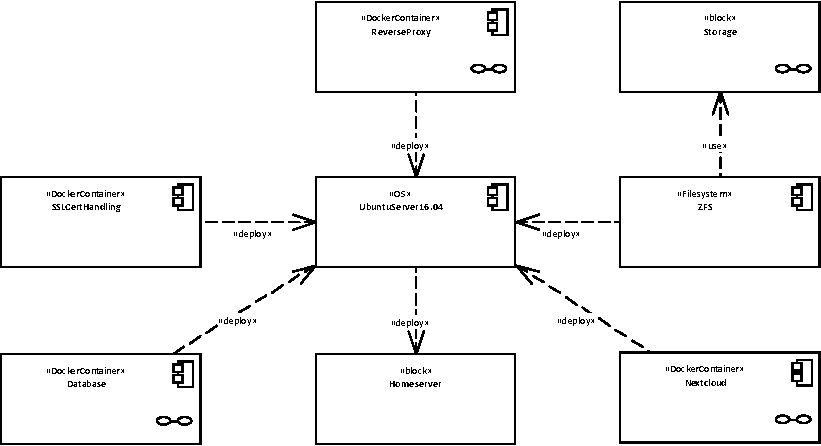
\includegraphics[scale=1]{durchfuehrung/figures/DeploymentOS}
  \caption[Deployment-Diagramm Applikationen und OS]{Komponentendiagramm der
    eingesetzten Softwarekomponenten und ihre Beziehung zum Betriebssystem. Die
    Abh�ngigkeit stereotypisiert mit $\ll$deploy$\gg$ bedeutet hierbei, dass die
    Komponente die jeweilige Ziel\-komponente als Laufzeitumgebung nutzt.}
  \label{fig:deplos}
\end{figure}

\newpage

Das Deployment der Anwendungen selbst erfolgt dann auf die Docker-Container, wie
in Abbildung \ref{fig:depldb} gezeigt. Je nach Konfiguration findet die
Anwendung ein vollst�ndiges Betriebssystem mit allen Abh�ngigkeiten vor, die im
Dockerfile definiert wurden.

\begin{figure}[h]
  \centering
  
\includegraphics{durchfuehrung/figures/DeploymentDB}
  
\includegraphics{durchfuehrung/figures/DeploymentRP}
  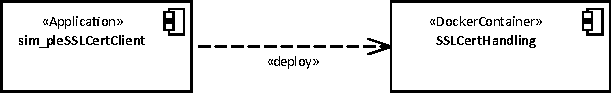
\includegraphics{durchfuehrung/figures/DeploymentSSL}
  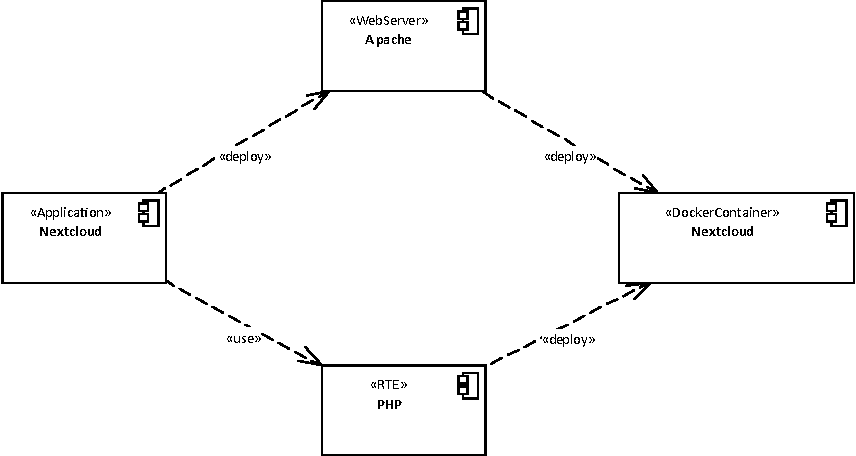
\includegraphics[scale=0.8]{durchfuehrung/figures/DeploymentNC}
  \caption[Deployment-Diagramm Anwendungen]{Deployment der Anwendungen auf die
    dazugeh�rigen Docker-Container}
  \label{fig:depldb}
\end{figure}


\subsection{Starten der Docker-Container}
\label{sec:sw_arch_start}

Die einfachste M�glichkeit, einen Docker-Container zu starten, ist die Eingabe
des Befehls \texttt{docker run <image\_name>}. Ein Image ist ein mit
\texttt{docker build} gebautes Dockerfile vergleichbar mit dem Image eines
Betriebssystems. Mit dem \texttt{docker run} Befehl wird dieses gestartet und es
entsteht die Instanz eines Images, ein Container. Mehr Informationen zum Befehl \texttt{docker run} ist in \cite{docker_run_reference} zu finden.

Die beschriebene Methode ist f�r einfache Tests gut verwendbar. Ist jedoch ein
komplexes Gebilde aus Containern zu bauen, so ist es nicht zielf�hrend bei jedem
Start alle Container von Hand zu starten. Hierf�r wird von Docker das Werkzeug
Docker Compose bereit gestellt. Dieses liest eine Datei aus (standardm��ig
\texttt{docker-compose.yml}), in der alle Optionen definiert sind, mit denen die
Container sonst mit \texttt{docker run} gestartet werden. Mehr Informationen zu Docker Compose sind in \cite{docker_compose_reference} zu finden.

Im hier vorgestellten System wurde eine \texttt{docker-compose.yml}-Datei f�r
Basisdienste wie die Datenbank und den Reverse Proxy, sowie eine Datei f�r die
konkrete Anwendung wie die Nextcloud. Dieses Verfahren erm�glicht eine getrennte
Verwaltung von Infrastruktur und Anwendung.

\newpage

\subsection{Interne Kommunikation der Container}
\label{sec:sw_arch_kom}

Um eine Kommunikation zwischen den Containern zu erm�glichen wird das Feature
\textit{network} von Docker genutzt. Dieses erm�glicht den Aufbau virtueller
TCP/IP-Netzwerke innerhalb einer Maschine (=\textit{Bridge}-Netzwerk) oder auch
maschinen�bergreifend (=\textit{Overlay}-Netzwerk) zum Aufbau von Clustern. Da jeder Container eine kleine virtuelle Maschine darstellt, verf�gt auch jeder Container �ber eine Netzwerkschnittstelle, mit der er dem ausgew�hlten Netzwerk beitreten kann.

Im vorliegenden Projekt wurden ausschlie�lich Bridge Netzwerke genutzt, da nur
eine Maschine vorhanden ist. Dabei wurden die Netzwerke \textit{frontend} und
\textit{backend} eingerichtet. Dies erm�glicht eine virtuelle Trennung zwischen
der Benutzerseite (z.B. der Reverse-Proxy, der Nutzeranfragen von au�en
verarbeitet) und dem Server-Backend (z.B. die Datenbank). Abbildung
\ref{fig:compsw} zeigt die Beziehung der Container untereinander.

\begin{landscape}

\begin{figure}[h]
  \centering
  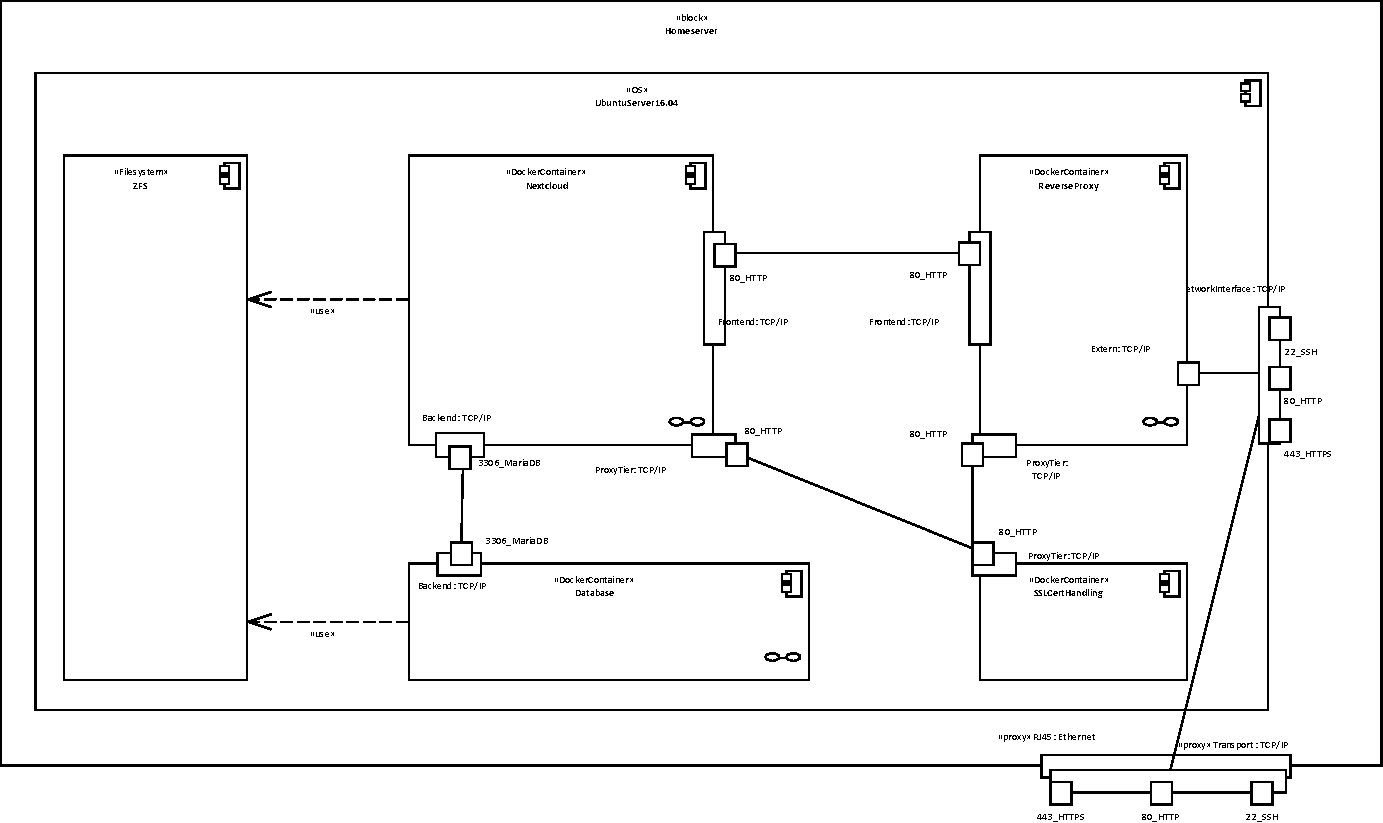
\includegraphics[angle=0, scale=1]{durchfuehrung/figures/CompositionSW}
  \caption[Kompositionsdiagramm der Docker-Container]{Kompositionsdiagramm der
    eingesetzten Docker-Container. Die Docker-Container sind jeweils �ber die
    passenden Bridge-Netzwerke \texttt{frontend} und \texttt{backend}
    miteinander verbunden. Die Datenbank und die Nextcloud nutzen den von ZFS
    verwalteten Speicherpool als Speicher-Backend}
  \label{fig:compsw}
\end{figure}

\end{landscape}



%%% Local Variables:
%%% mode: latex
%%% TeX-master: "../doku_server"
%%% End:
